
\documentclass{beamer}

\usepackage[T1]{fontenc}
\usepackage[utf8]{inputenc}
\usepackage[french,english]{babel}

\usepackage{lmodern}
\usepackage{amsthm}
\usepackage{float}
\usepackage{lmodern}%pour un meilleur rendu des polices
\usepackage{verbatim}%du texte non interprt
\usepackage{amsmath}
\usepackage{amssymb}%maths
\usepackage{xspace}
\usepackage[dvipsnames,svgnames,table]{xcolor}
\usepackage{listings}
\usepackage{fancyhdr}
\usepackage{etoolbox}
\usepackage{titlesec}
\usepackage{titletoc}
\usepackage{lastpage}
\usepackage{hyperref}
\usepackage{ctable} % for \specialrule command
\usepackage{cite}
\usepackage{algorithm2e}
\usepackage{alltt}
\usepackage{array}
\usepackage{mdwmath}
\usepackage{mdwtab}
\usepackage{eqparbox}
\usepackage{subfig}
\usepackage{dblfloatfix}
\usepackage{url}
\usepackage{tipa}
\usepackage{stmaryrd}
\usepackage{upgreek}
\usepackage{mathrsfs}
\usepackage{ulem}
\usepackage{cancel}

\graphicspath{{img/}}
\DeclareGraphicsExtensions{.pdf,.jpeg,.jpg,.png}


\newcommand{\ccite}[1]{\textbf{\cite{#1}}}
\newcommand{\pd}[2]{\dfrac{\partial #1}{\partial #2}}
\newcommand{\od}[2]{\dfrac{\mathscr{D}_a #1}{\mathscr{D} #2}}
\newcommand{\tensor}[1]{\mathbf{#1}}
\renewcommand{\vector}[1]{\overrightarrow{#1}}

\newcommand{\Tau}{\tensor{\mathlarger{\uptau}}}
\renewcommand{\v}{\vector{u}}
\newcommand{\W}{\tensor{W\left( \v \right)}}
\newcommand{\D}{\tensor{D\left( \v \right)}}
\newcommand{\grad}{\vector{\nabla}}
\newcommand{\gradv}{\tensor{\nabla\v}}
\renewcommand{\div}[1]{div \left( #1 \right)}
\newcommand{\divv}[1]{\vector{div} \left( #1 \right)}
\newcommand{\UU}{\mathcal{U}}
\newcommand{\VV}{\mathcal{U}}
\newcommand{\M}{\mathcal{M}}
\newcommand{\A}[2]{\mathcal{A}_{#1}\left( #2 \right)}
\newcommand{\Uu}{\UU^{n}}
\newcommand{\Uv}{\UU^{n+\theta}}
\newcommand{\Uw}{\UU^{n+1-\theta}}
\newcommand{\Ux}{\UU^{n+1}}
\newcommand{\Uk}{\UU^{k}}
\newcommand{\Ukk}{\UU^{k+1}}
\newcommand{\Vk}{\VV^{k}}
\newcommand{\Vkk}{\VV^{k+1}}
\newcommand{\Tauk}{\Tau^{k+1}}
\newcommand{\vk}{\v^{k+1}}
\newcommand{\pk}{p^{k+1}}
\newcommand{\Dk}{\tensor{D\left( \vk \right)}}

\definecolor{lightgray}{gray}{0.9}
\definecolor{titlecolor}{RGB}{0,0,200}
\definecolor{subtitlecolor}{RGB}{0,0,153}
\definecolor{textcolor}{RGB}{0,128,255}
\definecolor{RoyalPurple}{RGB}{102,51,153}
\definecolor{ForestGreen}{RGB}{34,139,34}


\newcommand{\colbox}[1]{\colorbox{lightgray}{$ #1 $}}

\newcommand{\stitle}[2][0.3cm] { 
    {\normalsize \textcolor{titlecolor}{\textbf{#2}}} 
    \vspace{#1} 
}

\newcommand{\ssubtitle}[1]{ {\footnotesize \textcolor{subtitlecolor}{\textbf{#1}}} }

\newcommand{\stress}[1]{\textcolor{textcolor}{#1}}

\newcommand{\hidecontent}[2][0.25]{{% \hidecontent[<transparency>]{<stuff>}
  \setbox9=\hbox{#2}% Store <stuff> in \box9 to obtain height/width
  \transparent{#1}\ooalign{\usebox9\cr\color{white}\rule{\wd9}{\ht9}\cr}}}


\begin{document} 

\maketitle 
\tableofcontents

\section{Introduction}

This is a partial implementation of Christophe P. Bernard thesis on interpolating Deslauriers and Dubuc wavelets.

\vskip 0.5cm
\noindent \textbf{The implementation concists in three main parts :}

\begin{itemize}
    \item A maple script to generate low pass filter coefficients $h_n$ and Deslauriers-Dubuc wavelets (1D, 2D).
    \item Python scripts to generate Deslauriers-Dubuc wavelet families on the interval.
    \item Final efficient implementation of the method in one dimension written in C++.
\end{itemize}

\clearpage
\section{Folder architecture}

\renewcommand*\DTstylecomment{\color{black}}
\renewcommand*\DTstyle{\ttfamily\textcolor{red}}

Here is an synthetic overview of given files :
\vskip 0.3cm

\dirtree{%
.1 \textbf{Root folder}.
.2 \textit{readme.pdf}\DTcomment{This file !}.
.2 \textit{CMakeLists.txt}\DTcomment{CMake configuration file for C++}.
.2 \textbf{src/}\DTcomment{Contains all C++ sources and headers}.
.2 \textbf{build/}\DTcomment{Used to compile C++}.
.2 \textbf{modules/}\DTcomment{CMake helpers}.
.2 \textbf{scripts/}\DTcomment{Contains all maple and python scripts}.
.2 \textbf{papers/}\DTcomment{Contains the thesis and paper about implemented method}.
.2 \textbf{results/}\DTcomment{Contains some precomputed results}.
.2 \textbf{slides/}\DTcomment{Contains slides pdf, tex and images}.
}

\section{Original papers}

The original thesis and paper can be found in the following folder :

\vskip 0.3cm

\dirtree{%
.1 \textbf{Root folder}.
.2 \textbf{papers/}.
.3 \textit{paper.pdf}\DTcomment{Short introduction paper on the proposed method}.
.3 \textit{these.pdf}\DTcomment{Original PhD Thesis on the method, see pages 151 to 231}.
}

\section{Slides}

Slides of the presentation can be found at the following locations :
\vskip 0.3cm

\dirtree{%
.1 \textbf{Root folder}.
.2 \textbf{slides/}.
.3 \textit{slides.pdf}\DTcomment{Slides in pdf version}.
.3 \textit{*.tex}\DTcomment{Latex sources}.
.3 \textit{master.bib}\DTcomment{Bibliography}.
.3 \textbf{img/}\DTcomment{All images and animations used during presentation}.
}

\section{Scripts}

Here are the concerned files of this section :

\dirtree{%
.1 \textbf{Root folder}.
.2 \textbf{scripts/}\DTcomment{Contains all scripts}.
.3 \textit{wavelets.mw}\DTcomment{Maple script}.
.3 \textit{*.py}\DTcomment{Python scripts}.
}


\clearpage
\subsection{Maple script}

The maple script can generate the filter coefficients $h_n$ with Lagrange polynomials of any given order, it then iteratively compute Deslauriers and Dubuc wavelets with convolutions of the filter with a dirac. Finally it computes their Fourier transform and perform nice plotting. It was only tested with maple 18.

\vskip 0.3cm
{\large \textbf{Running the script :}} \textrm{\tild maple scripts/wavelets.mw}

\vskip 0.3cm
{\large \textbf{Parameters :}}
\begin{itemize}
    \item \textbf{Pmin :} Minimal Deslauriers-Dubuc order to generate (default = 1)
    \item \textbf{Pmax :} Minimal Deslauriers-Dubuc order to generate (default = 4)
    \item \textbf{levels :} Number of convolutions used to generate the wavelets (default = 4)
\end{itemize}


\vskip 0.3cm
{\large \textbf{Output overview :}}

\begin{figure}[H]
    \centering
   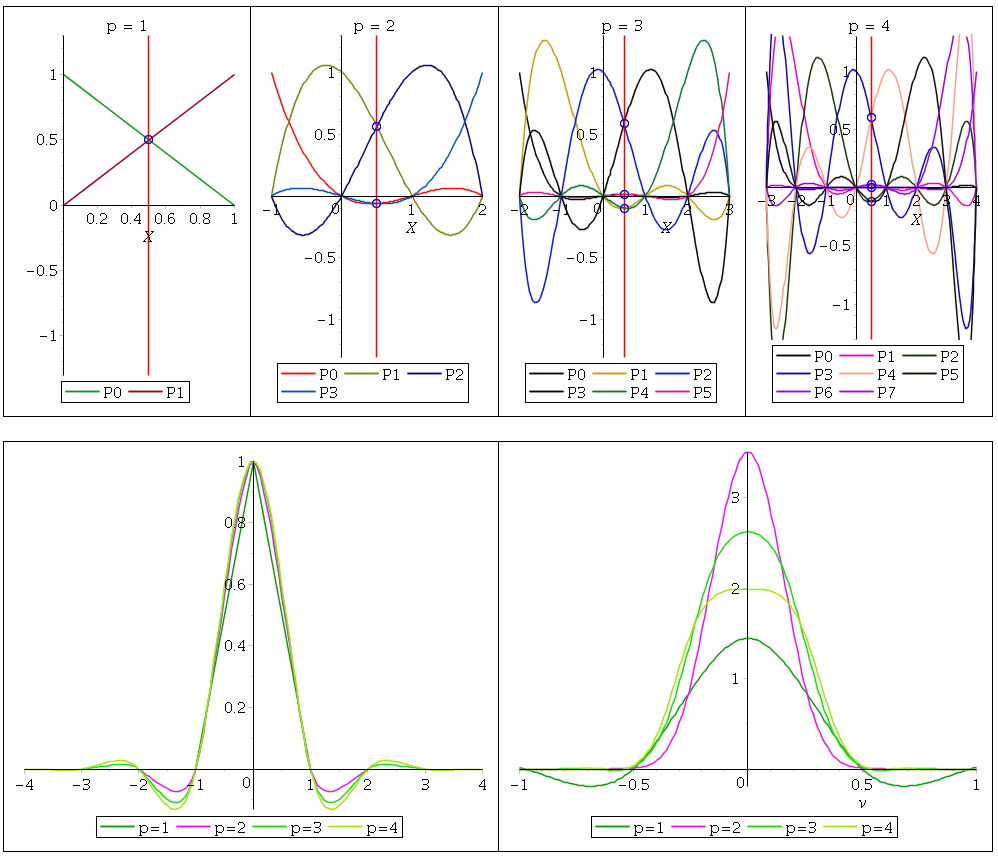
\includegraphics[scale=0.4]{maple}
   \caption{Output of the maple script $wavelets.mw$}
\end{figure}

\clearpage
\subsection{Python scripts}

    Python scripts can generate Deslauriers-Dubuc wavelet families on the interval as well as Deslauriers and Dubuc wavelet alone.
    It was coded and tested with python 2.7.6.

\vskip 0.3cm
    
    {\large \textbf{There are 3 scripts :}}

    \begin{itemize}
        \item \textbf{scripts/plot.py} : to plot 1D wavelets
        \item \textbf{scripts/plot2D.py} : to plot 2D wavelets
        \item \textbf{scripts/plotFamilies.py} : to plot wavelet families at a given level j on the interval $\Omega = [0,1]$
    \end{itemize}

\vskip 0.3cm
{\large \textbf{Running a script :}} \textrm{\tild python <script name>}

\vskip 0.3cm
{\large \textbf{Parameters :}} See comments in code.

\vskip 0.3cm
{\large \textbf{Output overview :}}

\begin{figure}[H]
    \centering
    \parbox{7cm}{
        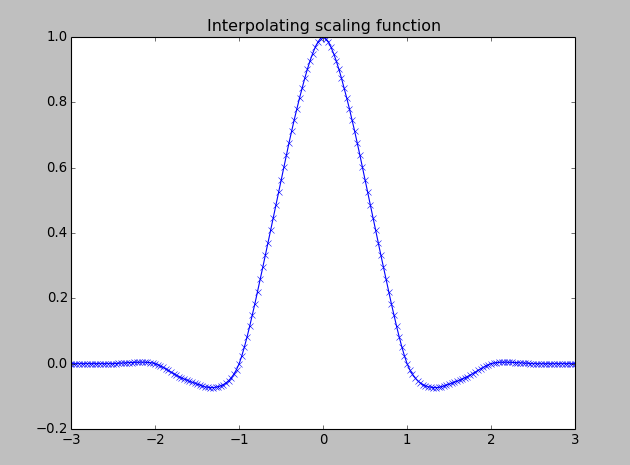
\includegraphics[width=7cm]{python1}
        \caption{Output of $plot.py$}
    }
    \qquad
    \begin{minipage}{7cm}
        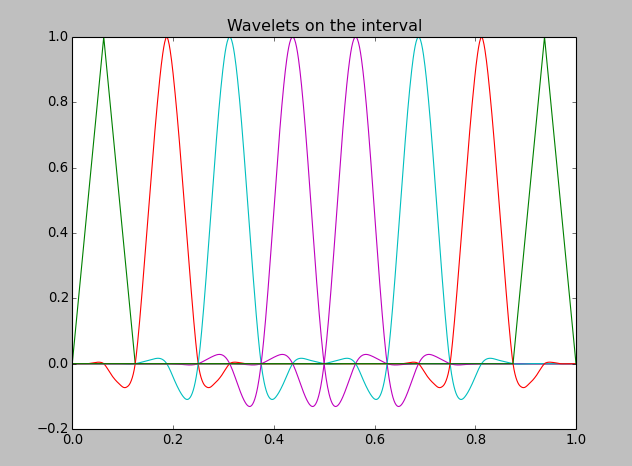
\includegraphics[width=7cm]{python2}
        \caption{Output~of~$plotFamilies.py$}
    \end{minipage}
\end{figure}

\begin{figure}[H]
    \centering
   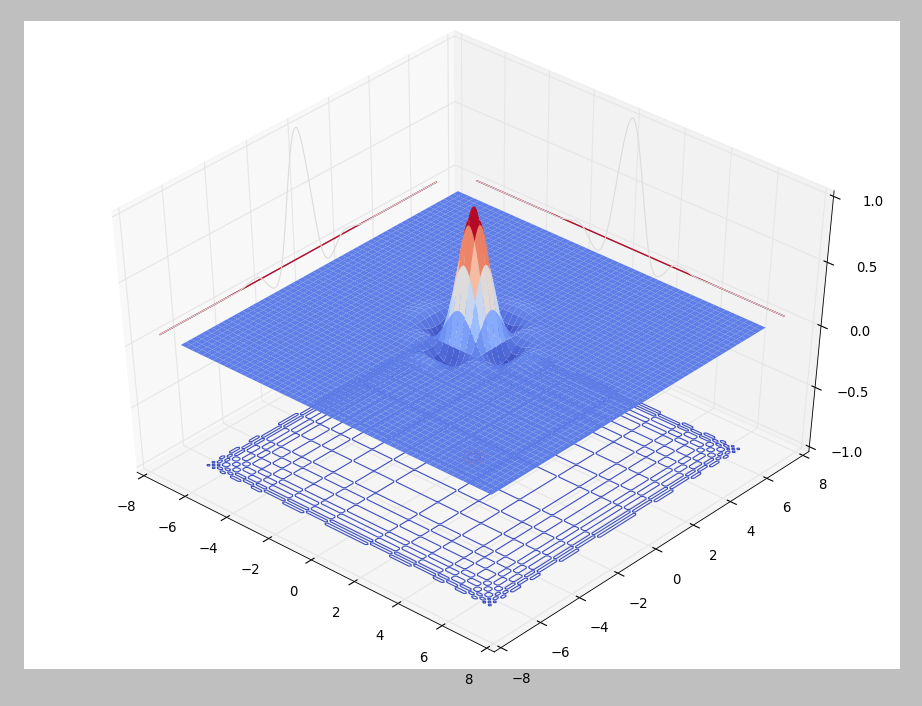
\includegraphics[scale=0.3]{python3}
   \caption{Output of $plot2d.py$}
\end{figure}

\clearpage
\section{Method implementation}

The full one dimensional method has been implemented in C++. It consists into three executables :
\begin{itemize}
    \item \textbf{main :} Apply and plot the intermediate steps of the proposed interpolation method.
    \item \textbf{bench :} Benching code to check efficiency and check interpolation error in $\ell_2$ and $\ell_\infty$ norm.
    \item \textbf{animation :} Executable to generate incremental sample interpolation animations (generate gif files).
\end{itemize}

\subsection{Dependencies}

\textbf{To compile you need a Unix like distribution and a C++11 capable compiler} : Tested with gcc 4.8.2 on Linux Mint 17 Qiana.

\vskip 0.3cm
It should work on a Mac but it has not been tested.

\vskip 0.3cm
The following libraries are required for the compilation of the C++ sources :

\begin{itemize}
    \item Console Gnuplot (C++ wrapper $/src/gnuplot/gnuplot.hpp$) 
    \item Eigen3 (for linear system solving)
    \item Boost (mainly for the gnuplot wrapper)
        \begin{itemize}
                \item System 
                \item Filesystem 
                \item Iostreams
        \end{itemize}
    \item ImageMagick (to generate gifs)
        \begin{itemize}
            \item MagickCore 
            \item Magick++
        \end{itemize}
\end{itemize}

\subsection{Compiling}

The three executables ($main$, $bench$ and $animation$) can be generated with the following commands :
\vskip 0.3cm

\noindent\textbf{In normal mode :} \\
\textrm{\tild\ cd build/} \\
\textrm{\tild\ cmake ..} \\
\textrm{\tild\ make -j8}

\vskip 0.3cm
\noindent\textbf{In debug mode (add debugging symbols):} \\
\textrm{\tild\ cd build/} \\
\textrm{\tild\ cmake -DCMAKE\_BUILD\_TYPE=Debug ..} \\
\textrm{\tild\ make -j8}

\clearpage
\noindent\textbf{In release mode (enable optimizations): } \\
\textrm{\tild\ cd build/} \\
\textrm{\tild\ cmake -DCMAKE\_BUILD\_TYPE=Release ..} \\
\textrm{\tild\ make -j8}

\vskip 0.3cm
\noindent Executables will be generated directly in the \textbf{build/} directory.
\vskip 0.3cm
\textbf{Execution :} \textrm{\tild\ ./<executable name>}
    
\subsection{Main program}
    Apply and plot the intermediate steps of the proposed interpolation method.
    See comments in the code.

    \vskip 0.3cm
    \textbf{Overview :}
    
    \begin{figure}[H]
    \centering
    \parbox{7cm}{
        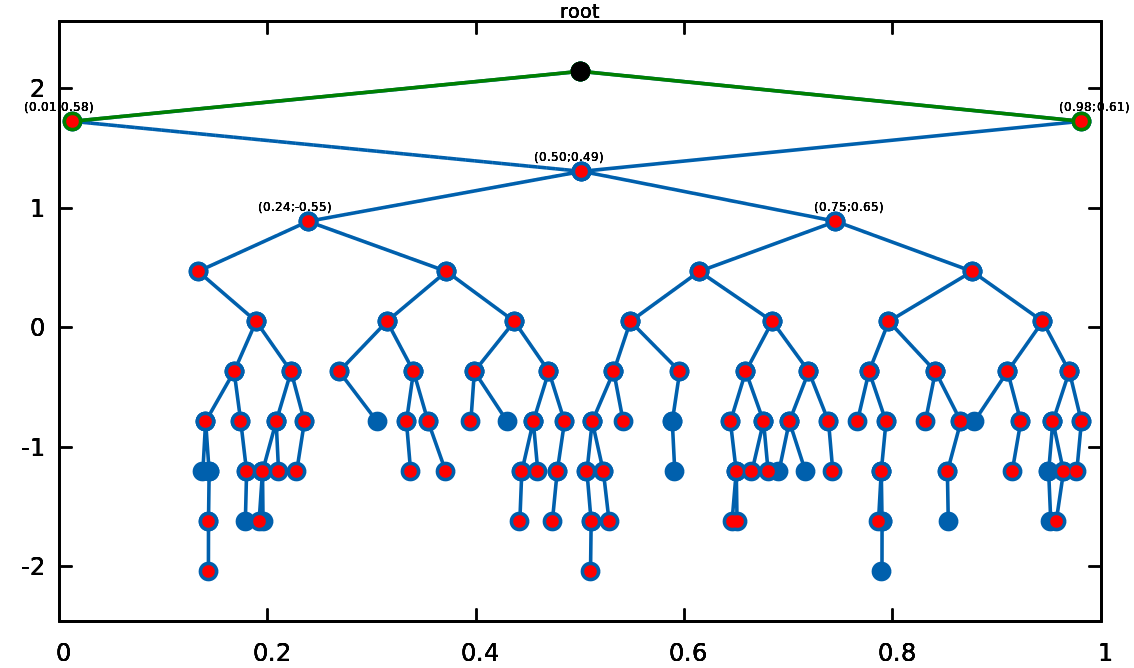
\includegraphics[width=7cm]{main_1}
        \caption{Constructed wavelet tree and extracted subtree.}
    }
    \qquad
    \begin{minipage}{7cm}
        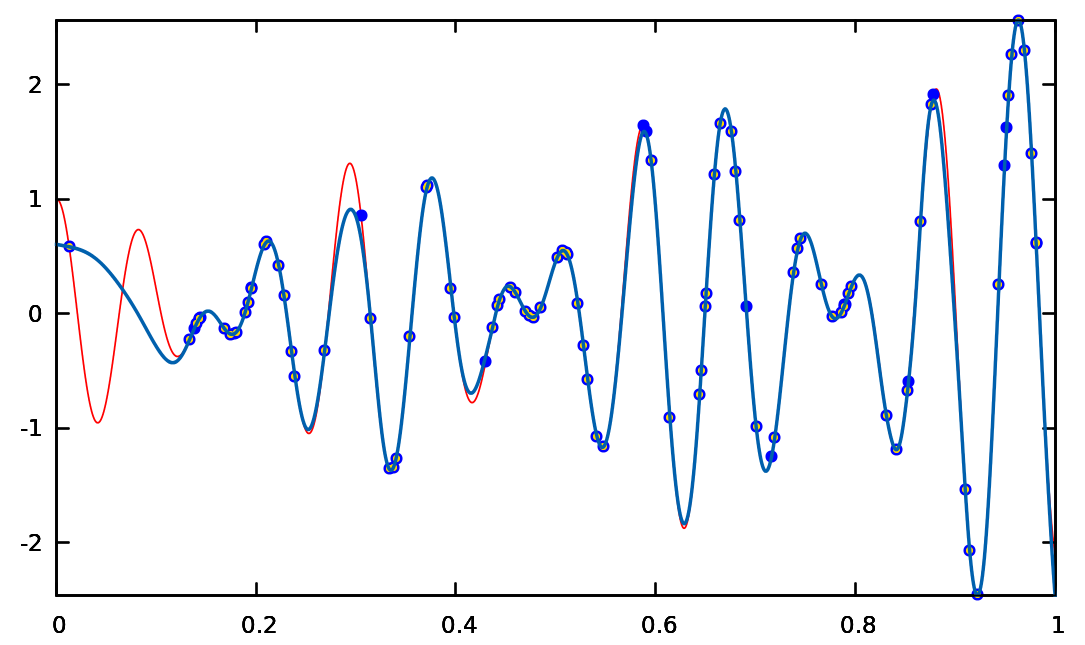
\includegraphics[width=7cm]{main_2}
        \caption{Interpolated function in red, result of the interpolation in blue.}
    \end{minipage}
\end{figure}


\subsection{Benching program}
    Benching code to check efficiency and check interpolation error in $\ell_2$ and $\ell_\infty$ norm.
    See comments in the code.

    \vskip 0.3cm
    \noindent Results of the run on my computer as well as some graphics are available in folder $results/$.
\subsection{Animation program}
    Executable to generate incremental sample interpolation animations (generate gif files).

    \vskip 0.3cm
    \textbf{Overview :} See $slides/img/interpolation.gif$ for an example, see comments in the source code to generate your own gifs.

\clearpage
\subsection{Source code overview}

Here are the source files of the C++ implementation :

\vskip 0.3cm

\footnotesize
\dirtree{%
.1 \textbf{Root folder}.
.2 \textit{CMakeLists.txt}\DTcomment{CMake configuration file for C++}.
.2 \textbf{build/}\DTcomment{Used to compile C++}.
.2 \textbf{modules/}\DTcomment{CMake helpers}.
.2 \textbf{src/}\DTcomment{Contains all C++ sources and headers}.
.3 \textit{main.cpp}.
.3 \textit{bench.cpp}.
.3 \textit{animation.cpp}.
.3 \textbf{gnuplot}\DTcomment{Contains gnuplot utilities}.
.4 \textit{gnuplot.hpp}\DTcomment{C++ header only gnuplot wrapper library}.
.4 \textit{affineTransformation.hpp}.
.4 \textit{plotBox.hpp}.
.4 \textit{plotUtils.hpp}.
.3 \textbf{sample}\DTcomment{Contains sample structures}.
.4 \textit{point.hpp}.
.4 \textit{sample.hpp}.
.4 \textit{functionSample.hpp}.
.4 \textit{randomSample.hpp}.
.3 \textbf{tree}\DTcomment{Contains tree structures}.
.4 \textit{treeNode.hpp}.
.4 \textit{integerGrid.hpp}.
.4 \textit{binaryTreeNode.hpp}.
.4 \textit{waveletTree.hpp}.
.3 \textbf{wavelets}\DTcomment{Contains wavelet related structures}.
.4 \textit{interval.hpp}.
.4 \textit{wavelet.hpp}.
.4 \textit{deslaurierDubuc.hpp}.
.4 \textit{deslaurierDubucUtils.hpp}.
.4 \textit{waveletMapper.hpp}.
.3 \textbf{utils}\DTcomment{Mainly utilities : constants, vector, random, ...}.
.4 \textit{config.hpp.in}\DTcomment{Cmake configured header input}.
.4 \textit{config.hpp.out}\DTcomment{Cmake configured header output (created at compile time)}.
.4 \textit{consts.hpp}.
.4 \textit{defines.hpp}.
.4 \textit{globals.hpp}.
.4 \textit{headers.hpp}.
.4 \textit{utils.hpp}.
.4 \textbf{maths}\DTcomment{Vector and Matrix}.
.5 \textit{vec.hpp}.
.5 \textit{vec2.hpp}.
.5 \textit{vec3.hpp}.
.5 \textit{vecBool.hpp}.
.5 \textit{matrix.hpp}.
.4 \textbf{random}\DTcomment{Random number generation utility}.
.5 \textit{rand.hpp}.
}


\end{document}




 
 
 
 
 
 
 
 
 
 
 
 
